\textnormal{
In this stage, we specify the flow of our system by showing steps in data curation, how we plan to implement classifiers and use its model for prediction as well as the Regression model and connect this with the classifier model. Then, we show how each model is generated by looking at the high level pseudo code for the classifier and the regressor and detail how it is to be implemented. We also specify the data structures that are to be used and take a look at the expected time and space complexity for the same.\\ }
\begin{itemize} 
\item{  System Flow Description. }
The system utilizes the flights training data to develop the models. At the first step, the classifiers takes the flights data as input and create a model that is stored in the disk. This model is then used for predicting if any given flight is to be classified as on-time or delayed. For all the flights classified as delayed, we develop a regression model at the next step and store this model in the disk. This model will help us to estimate by how much time any given flight is delayed. The following two flowcharts explores the system flow chart at high level between the two major components of this system, classifier and regressor. The Fig. 1 flowchart details about generating the classification model and then based on its model conditions when we implement the regressor. The Fig. 2 flowchart details what the flow is when any user enters any input to the system. Here, the models stored in the disk during the earlier stage are utilized for prediction.  
\begin{figure}
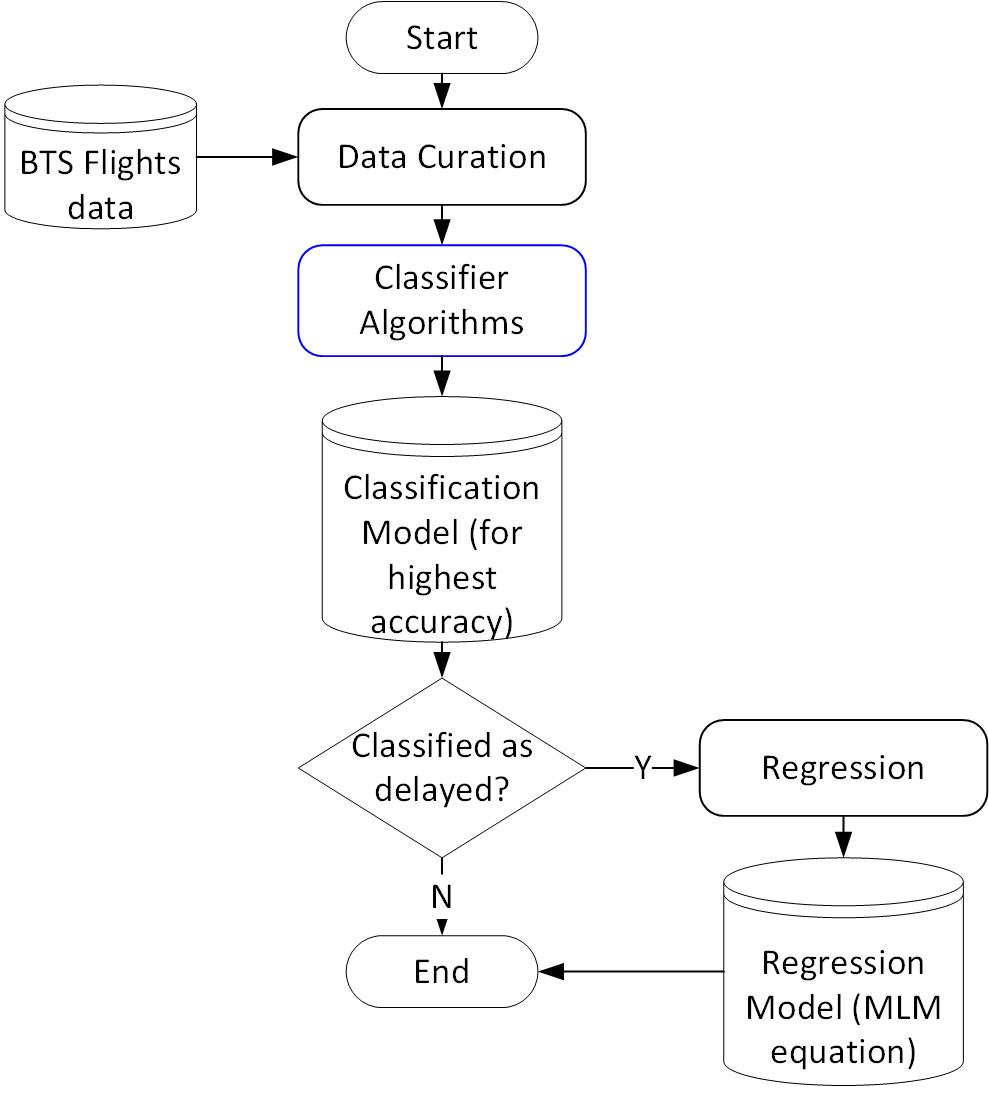
\includegraphics[height=230pt,width=\linewidth]{ModelGen.jpg}
\caption{Flow Diagram for generating Classification and Regression Models.}
\end{figure}
\begin{figure}
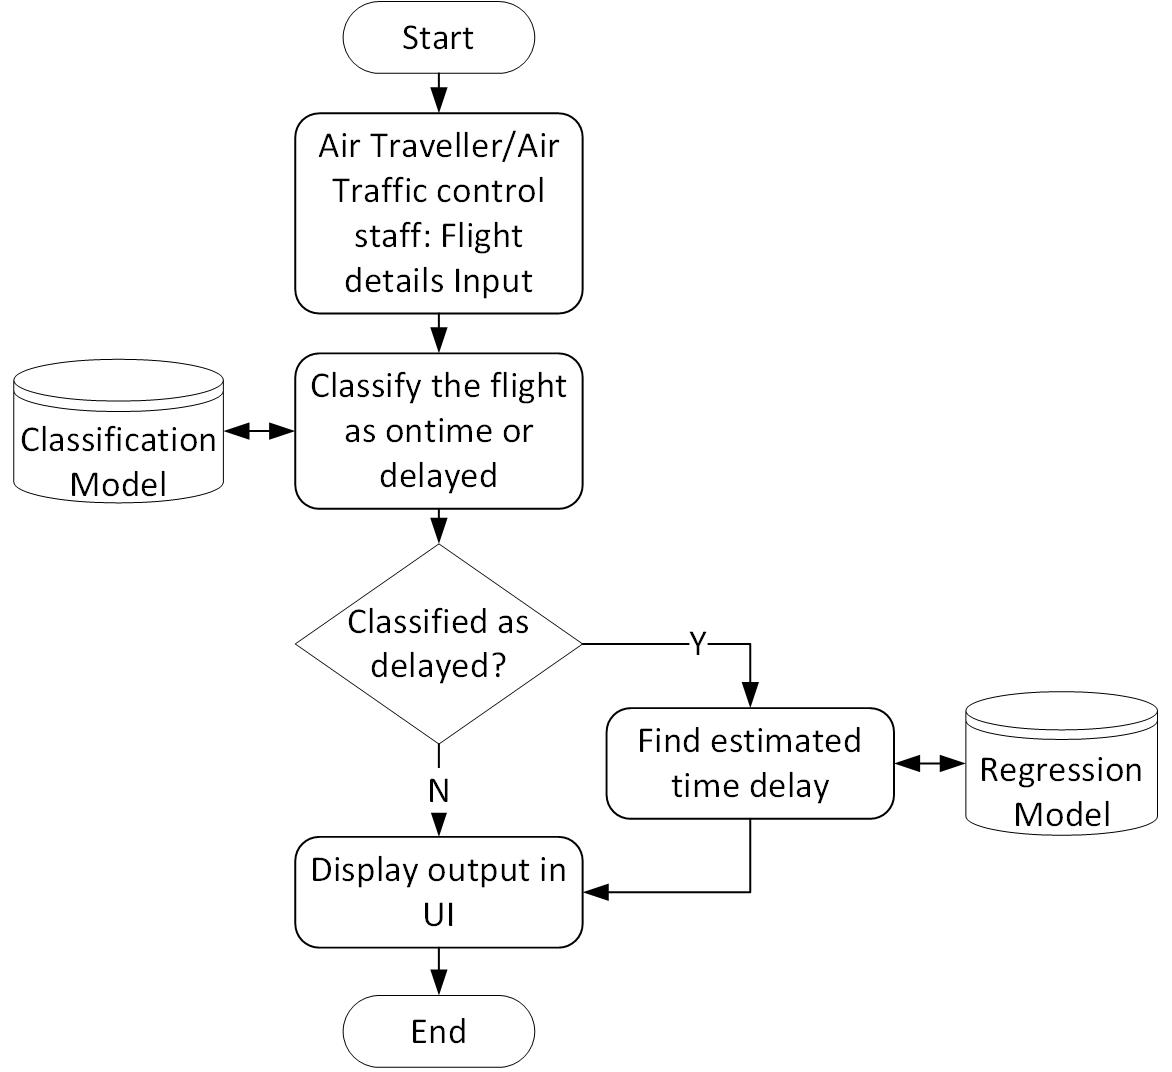
\includegraphics[width=\linewidth]{UserIP.jpg}
\caption{Flow Diagram for making predictions after taking the user input.}
\end{figure}
\\
\\
\\
\item{ High Level Pseudo Code of the system. }
$\\Begin:$

\begin{enumerate}
\item{$data\ =\ read(BTS\_flight\_data)$}
\item{$data \gets Data\_Curation(data)$}
\item{$classes\ =\ \{on\ time,\ delayed\}$}
\item{$Classification(data,classes)$}
\item{$data\_delayed \gets data\ classified\ as\ delayed$}
\item{$Linear\_Regression(data\_delayed)$}
\end{enumerate}
$End\\\\$
\item{Major Algorithms/Components in the Pseudo-code: }
\begin{enumerate}
\item{Data Curation: }
In this algorithmic component, we make sure that the data given as input to the classifier is curated. This is to try and make the classifier as accurate as possible. Following steps detail what actions we plan to take to curate the data.
\begin{itemize}
\item{ Remove records from csv file for which a field is empty (Incomplete records)}
\item{ Create 2 copies of dataset 
\\	1. Numeric : Preserves numeric values 
\\	2. Discretized : Maps Distance, Departure, Arrival time into intervals
\\\textit{Distance}: 
\\Assign interval id from 1 to 11 based on the distance covered(1: 0 to 250 miles, 2: 250 to 500 miles......11: 2500 to 2750 miles)
\\\textit{DEPARTURE TIME, ARRIVAL TIME}: 
\\Assign interval id from 1 to 3 based on the time of day(1: 12am to 8pm, 2: 8pm to 4pm, 3: 4pm to 12am)
}
\item{Randomize the records using WEKA}
\item{Remove flights with uncommon attribute values in ORIGIN/DESTINATION by choosing the Top 25 frequently occurring airports and discarding records for other airports}
\item{Remove flights with uncommon attribute values in CARRIER by choosing only Top 8 commercial airlines and discarding records for other airlines}
\item{Resample the data using WEKA}
\item{Divide the dataset into TRAINING and TESTING dataset in 3:1 ratio}
\end{itemize}

\item{Classifier: We use two main types of classifiers, namely Naive Bayes Tree and J48 Decision Trees. Apart from these, we also use Random Forest, Rule-based classifier and Simple Naive Bayes classifier for comparisons.}
\begin{itemize}
\item{Naive Bayes Tree Algorithm: This algorithm is similar to the classical recursive partitioning schemes, except that the leaf nodes created are Naive-Bayes categorizers instead of nodes predicting a single class. A threshold is chosen using decision trees and the utility of a node is computed by discretizing the data and computing the 5-fold cross-validation accuracy estimate of using Naive-Bayes at the node. The utility of a split is the weighted sum of the utility of the nodes, where the weight given to a node is proportional to the number of instances that go down to that node. The algorithm is as follows:}
\vspace{2.5 mm}
\\*Input: a set $T$ of labeled instances.
\\*Output: a decision tree with Naive-Bayes categorizers at the leaves.
\vspace{0.1 mm}
\begin{itemize}
\item{For each attribute $X_{i}$ evaluate the utility, $u(X_{i})$ of a split on attribute $X_{i}$. For continuous attributes, a threshold is also found at this stage.}
\item{Let $j = $ arg max$_{i}$$(u_{i})$, $i.e.$, the attribute with the highest utility.}
\item{If $u_{j}$ is not significantly better than the utility of the current node, create a Naive-Bayes classifier for the current node and return.}
\item{Partition $T$ according to the test on $X_{j}$. If $X_{j}$ is continuous, a threshold split is used; if $X_{j}$ is discrete, a multi-way split is made for all possible values.}
\item{For each child, call the algorithm recursively on the portion of $T$ that matches the test leading to the child.}
\end{itemize}

If there are $m$ instances, $n$ attributes and $l$ label values, the complexity of the attribute selection phase for discretized attributes is $O(m.n^{2}.l)$. In our case, the number of attributes is less than $O$(log$m$) and the number of labels is small. Hence the time spent on attribute selection using cross-validation is less than the time spent sorting the instances by each attribute. Thus NBTree scales up well to our large database.
\vspace{2.5 mm}
\item{J48 Decision Trees: J48 is an open source implementation of the C4.5 machine learning algorithm which creates decision trees based on the ID3 algorithm, using information entropy and information gain. Entropy is a measure of unpredictability of information content and expected information gain is the change in information entropy $H$ from a prior state to a state that takes some information as given: $IG(T,a) = H(T) - H(T|a)$. This algorithm has a few base cases:
\begin{itemize}
\item{All the samples in the list belong to the same class. When this happens, it simply creates a leaf node for the decision tree saying to choose that class.}
\item{None of the features provide any information gain. In this case, C4.5 creates a decision node higher up the tree using the expected value of the class.}
\item{Instance of previously-unseen class encountered. Again, C4.5 creates a decision node higher up the tree using the expected value.}
\end{itemize} 
The C4.5 or J48 algorithm is as follows:}
\vspace{2.5 mm}
\\*Input: Training data set $S = {s_1, s_2, ...}$ of already classified samples. Each sample  $s_i$ consists of a p-dimensional vector $(x_{1,i}, x_{2,i}, ...,x_{p,i})$ , where the  $x_j$  represent attribute values or features of the sample, as well as the class in which  $s_i$  falls.
\\*Output: Decision tree
\vspace{0.1 mm}
\begin{itemize}
\item{Check for base cases}
\item{For each attribute $a$ Find the normalized information gain ratio from splitting on $a$}
\item{Let $a_{best}$ be the attribute with the highest normalized information gain}
\item{Create a decision node that splits on $a_{best}$}
\item{Recur on the sublists obtained by splitting on $a_{best}$, and add those nodes as children of node}
\end{itemize}

\item{Random Forest: Random forests is a notion of the general technique of random decision forests that are an ensemble learning method for classification, regression and other tasks, that operate by constructing a multitude of decision trees at training time and outputting the class that is the mode of the classes (classification) or mean prediction (regression) of the individual trees. Random decision forests correct for decision trees' habit of overfitting to their training set.}

\item{Rule-based classifier: Rule-based classifier makes use of a set of $IF-THEN$ rules for classification. One rule is created for each path from the root to the leaf node. To form a rule antecedent(the $IF$ part), each splitting criterion is logically $ANDed$. The leaf node holds the class prediction, forming the rule consequent(the $THEN$ part). Such rules are then extracted using a sequential covering algorithm and then pruned due to the following reasons: }
\begin{itemize}
\item{Assessment of quality is made on the original set of training data. The rule may perform well on training data but less well on subsequent data. Hence rule pruning is required.}
\item{The rule is pruned by removing conjunct. A rule R is pruned, if pruned version of R has greater quality than what was assessed on an independent set of tuples.}
\end{itemize}

\item{Simple Naive Bayes classifier: Naive Bayes classifier is a simple probabilistic classifier which is based on Bayes theorem with strong and naive independence assumptions. In other words, Bayes' theorem is used in the classifier's decision rule.  Despite the naive design and oversimplified assumptions that this technique uses, Naive Bayes performs well in many complex real-world problems.
Even though it is often outperformed by other techniques such as boosted trees, random forests, Max Entropy, Support Vector Machines etc, Naive Bayes classifier is very efficient since it is less computationally intensive (in both CPU and memory) and it requires a small amount of training data. Moreover, the training time with Naive Bayes is significantly smaller as opposed to alternative methods.
Its performance is very close to more complicated and slower techniques in many cases.}
\end{itemize}

\item{Linear Regression:}
In this component, we obtain the multiple linear regression model as a linear relationship between the delay in time acting as our response variable and the attributes of the flight like departure airline, airport, departure time, etc. acting as our explanatory variables. For our regressor, we represent these attributes as a matrix of features $(X_{n\times m})$ for all flights. $X_{ij}$ denotes the $j^{th}$ feature of the $i^{th}$ flight record.
\[
X_{n\times m} =
\begin{bmatrix}

X_{11} & X_{12} & ... & X_{1m} \\
X_{21} & X_{22} & ... & X_{2m} \\
... \\
... \\
X_{n1} & X_{n2} & ... & X_{nm}
\end{bmatrix}
\]
Next, we formulate the delay in time $(Y_i)$ as follows. Note that $x_{im}$ is the $m^{th}$ feature of this flight and $\beta$s are the slope intercepts calculated in regression.\vspace{0.1cm}
\\
\text{\ \ \ \ \ $Y_i$ = $\beta _0$ + $\beta _1X_{i1}$ + $\beta _2X_{i2}$ + ... + $\beta _mX_{im}$}\vspace{0.1cm}
\\For any given details of the flight as entered by the user, we treat them as our x values in the above equation and find the corresponding Y value which is the estimated delay in time of the flight. This is the main output of this algorithm. It takes time complexity based on number of features $m$ and our total records of flight $n$. It comes to $\mathcal{O}(nm^2)$ for multiple linear regression.

\end{enumerate}
\end{itemize}

\begin{itemize} 
\item{ Major Integrity Constraints.}
This system has three main integrity constraints:\begin{itemize} 
\item{Data curation: }
The data given to the classifier must not have any null values and all attributes must be in their respective data type, whether numeric or string. 
\item{Classifier output: }
The classifier should predict with at least 60\% accuracy when testing with the validation data. Here, the regression must be calculated only for delayed flights and not otherwise.
\item{Regressor output: }
Regression must be carried out only for linear and homoscedastic data obtained from the classifier's output.
\end{itemize}
\end{itemize}